\section{The CC-Layer}
\label{sec:implement}
\subsection{Constructing the CC-layer}
\label{sec:implement_construct}
Given a discrete feature map $\varbold{I}$ of shape $[N,C_{in},H,W]$, we are interested in a layer that produces $\varbold{I'}=CC\{\varbold{I}\}$ of shape $[N,C_{out},H',W']$ which is resized by a (non-integer) scale-factor $(s_h, s_w)$. Here $N$ is the batch-size, $C$ is the number of channels. $H,W$ are spatial dimensions. The desired spatial size $H',W'$ may be chosen at inference time.
Our CC-layer consists of 4 principled building blocks, marked by numbers in Fig.~\ref{fig:overview} (for simplicity, $I$ and $I'$ are drawn as 2D vectors in Fig.~\ref{fig:overview}, i.e.,  4D tensors with $N=1$ and $C=1$). These are described next:

\textbf{Block 1 -- Projected-grid:} 
The Projected grid \varbold{$\textbf{g}$} matches each output `pixel' $\textbf{n}$=$(i', j')$$\in$$I'$ to a sub-`pixel' location \varbold{$\textbf{g}_n$} in the continuous space of the \ben{input} $I$. This grid is captured by a tensor of shape $[2,H',W']$ where the the first dimension are the 2 projected sub-`pixel' coordinates (vertical and horizontal) of each output `pixel' $\textbf{n}$=$(i', j')$$\in$$I'$, and $H', W'$ are for all the output `pixels'.

%\michal{why don't we see the number of Fig.4 in the next paragraph?}

Let's start with a simple example. Fig.~\ref{fig:grid}.a depicts a standard 1D  downscaling by %an integer 
$2$. Note that even when the scale-factor $s$ is an integer (or an inverse integer: ${s=\ben{\nicefrac{1}{2}}}$ in this case), it is  \emph{wrong} to map an output `pixel' position $\textbf{n}$$\in$$I'$  to its input position in $I$ by simply multiplying (or dividing)  by the scale-factor $s$. It can be observed in Fig.~\ref{fig:grid}.a   that ${\varbold{\textbf{g}_n}\neq2\textbf{n}=\textbf{n}}/{s}$
%\ben{\nicefrac{\textbf{n}}{s}}}$.
To obtain the correct mapping, let's
define $d_{out}$  to be the distance of any output `pixel'  
%\textbf{n}$$\in$$I'$  
\michal{$\textbf{n}$}
from the leftmost boundary of $I'$.  $d_{out}$  is measured in units of output `pixels'. The matching coordinates \varbold{$\textbf{g}_n$}   in the \ben{input} $I$  is  defined to have a distance $d_{in}$ from the leftmost boundary of  $I$, and is measured in units of input `pixels'. The correct mapping rule across image scales~\cite{MATLAB:2010} is $d_{in}$=${d_{out}}/{s}$, 
since the total shape (from boundary-to-boundary) is resized, rather than discrete `pixel' centers. Since the first `pixel' \emph{center} (in any \ben{feature map/image}) is always half a `pixel' away from the leftmost boundary, hence:
%we can easily relate $d$ to $n$ and to $\varbold{\textbf{g}_n}$, by 
$d_{out}$=$n$+$\frac{1}{2}$  and  $d_{in}$=$\varbold{\textbf{g}_n}$+$\frac{1}{2}$.
%Plugging it in, we get the
This entails the
well known relation used in image resizing methods~\cite{MATLAB:2010}: 
%$ \varbold{\textbf{g}_n}$=$\frac{n}{s}$+$\frac{1}{2}$$\left(\frac{1}{s}-1\right)$
$ \varbold{\textbf{g}_n}$=$\frac{n}{s}$+$\frac{1}{2}$$(\frac{1}{s}$-$1).$

% \michal{the next paragraph is very tedious, can and SHOULD be shortened substantially.}
% However, we need to handle also non-integer output shapes. Such an example is illustrated in Fig.~\ref{fig:grid}.b. Since images or feature-maps  can only be represented  by integer-sized vectors/tensors, we will usually (but not always) determine the size of the output layer to be $out\_size =\lceil s \cdot in\_size \rceil$, However, the intrinsic (non-integer) output size $s \cdot in\_size$ must be kept, as this is the true size of the output, while the integer size contains an extra sub-`pixel' margin. Fig.~\ref{fig:grid}.b shows a projected grid for resizing a $4 \times 4$ input layer by 0.6 and 1.4,  respectively. The final output size ($3 \times 6$) is larger than the intrinsic size ($2.4 \times 5.6$), due to the ceiling $\lceil * \rceil$ operation. 
% % To prevent misalignments, we need to map each output `pixel' center to its correct input `pixel' center. For this we need to shift the output `pixels' by half of the margin $\textbf{n}=\textbf{n}' -(out\_size - in\_size \cdot s)/2$. Plugging this into the relation of $p$ to $p'$ we obtain:
% To prevent misalignments due to this added sub-`pixel' output margin, and guarantee that each output `pixel' center is mapped to its correct input location, we need to shift the output `pixels' by half of the added margin:  $\textbf{n}=\textbf{n}' -(out\_size - in\_size \cdot s)/2$. %Plugging this into the relation of $p$ to $p'$ we obtain:
% This yields the final accurate grid mapping:
However, we need to handle also non-integer output shapes. The intrinsic output size 
$s \cdot in\_size$ may not be an integer, yet images or feature-maps  can only be represented  by integer-sized vectors/tensors. We will usually (but not always) determine the size of the output $I'$ to be $out\_size =\lceil s \cdot in\_size \rceil$. Fig.~\ref{fig:grid}.b shows an example of a projected grid for resizing a $4 \times 4$ input \ben{feature map} by scales 0.6 and 1.4,  respectively. The final output size ($3 \times 6$) is larger than the intrinsic size ($2.4 \times 5.6$), due to the ceiling operation $\lceil$*$\rceil$.  Therefore, the final  grid mapping (which accurately covers all cases) is:
\begin{align}
    \varbold{g_n} = \frac{n}{s} + \frac{1}{2}\Big( in\_size - 1\Big) - \frac{1}{2s}\Big(out\_size-1\Big)    
    \label{eq:grid}
\end{align}
% Since every output `pixel', (i, j) is mapped to continuous 2D coordinates in the input feature-map, % Since the grid matches two location coordinates to each output `pixel', 
% it is a represented as a standard CNN tensor of order 4, with shape $[1,2,H',W']$, where 
% the batch size is 1. The second dimension is 2 for 2 spatial continuous coordinates in the input space and the last two are for the height and width of the output. 


% First we calculate a grid of sub-pixel coordinates, which matches output pixels locations in the input continuous space. Each output pixel is assigned to horizontal and vertical sub-pixel position in the input. This grid is a function purely of the scale-factors and the output shape. Thus, importantly, the grid can be determined at inference time dynamically.

% To accurately obtain the projected-grid, we need to acknowledge that discrete `pixels' have non-infinitesimal size, thus we distinguish between `pixel' ordinal numbers to continuous locations of their centers. Fig.~\ref{fig:grid}.a depicts a 1d standard downscaling by a factor of $\frac{1}{2}$. Note that it even when the downscalinfg/upscalingis by an integer scale-factor (2 in this case), it is wrong to map output `pixel' positions to input positions by directly multiplying by the scale-factor. We mark the discrete `pixel' coordinates by $p$ and the scale-factor by $s$. First we observe that $p' \neq sp$. In the figure it is clear that `pixel' 0 should not be mapped to output `pixel' 0, rather the boundary between `pixel' 0 to `pixel' 1. We define the distance from the left boundary as $d$ measured in units of full `pixel's. Since the first `pixel' center is half a `pixel' to the right with respect to the left boundary, $d=p+\frac{1}{2}$. To correctly resize, we need the total size of the input (4 in the example) to be mapped to the total size of the output, hence $d'=s \cdot d$. plugging in the relation between $p$ and $d$: $p'+\frac{1}{2} = s(p+\frac{1}{2})$ so that the mapping rule between input and output `pixels' is $p = \frac{p'}{s} + \frac{1}{2} \left( \frac{1}{s} - 1 \right)$.


% Next we need to handle non-integer output shapes. Since we can only represent images or feature-maps sizes as integers we will usually (but not always) determine the output size as $Ceil(s \cdot in\_size)$. However, the intrinsic size $s \cdot in\_size$ must be held. We point out that in some cases of resizing, it is crucial to specify both scale-factors and output shape. For example, in a sequence of resizing operations. Fig.~\ref{fig:grid}.b illustrates projected grid for resizing by 0.6 and 1.4 respectively. The final output size is thus bigger than the intrinsic size. Depending on the kernel support, the output can be influenced by `pixels' out of the image, thus padding policy is required. Any further operation conducted on the output feature-map should treat the intrinsic size and not the padded size. The most reasonable convention in such cases is to preserve the center of the feature-map so that it maps to the center of the output. For this we need to shift the output `pixels' by half of the margin $p'=p'' -(out\_size - in\_size \cdot s)/2$. To finally obtain the grid, we map integer output `pixel' locations to their projected sub-`pixel' location in the input, we get for each dimension with its own scale-factor, input shape and output shape: 
% \begin{align}
%     g_n = \frac{n}{s} + \frac{1}{2}\Big( in\_size - 1\Big) - \frac{1}{2s}\Big(out\_size-1\Big)    
%     \label{eq:grid}
% \end{align}
% Since every output `pixel', (i, j) is mapped to continuous 2D coordinates in the input feature-map, % Since the grid matches two location coordinates to each output `pixel', 
% it is a represented as a standard CNN tensor of order 4, with shape $[1,2,H',W']$, where 
% the batch size is 1. The second dimension is 2 for 2 spatial continuous coordinates in the input space and the last two are for the height and width of the output. 

\begin{figure}
%\vspace*{-0.5cm}
    \centering
    \hspace{-3cm}
    \begin{minipage}{.5\textwidth}
      \centering
      \hspace{1cm}
      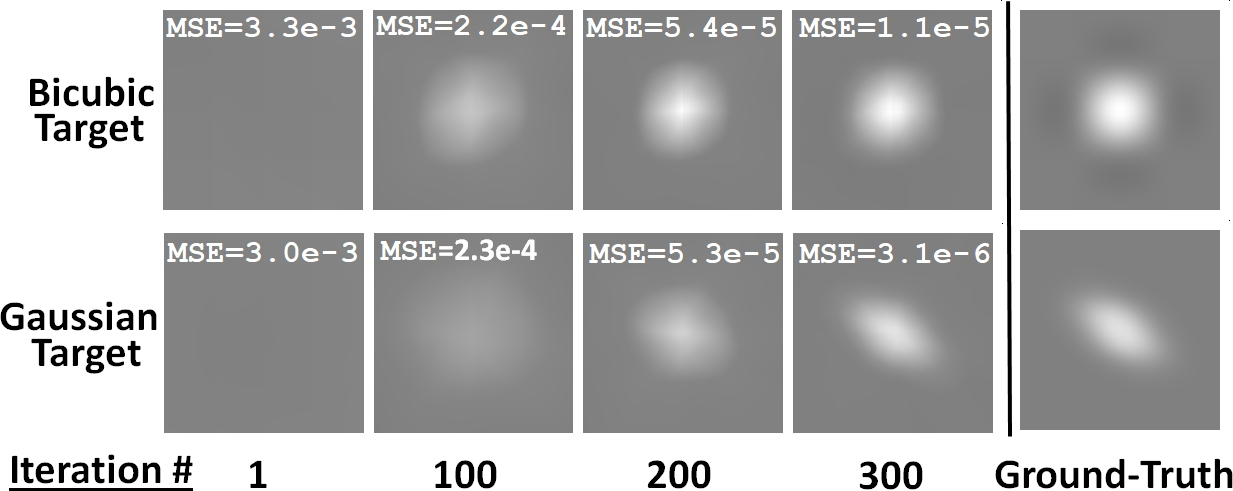
\includegraphics[width=1\textwidth]{figs/fig_visualize_Michal.jpg}
      \captionsetup{oneside, margin={-0.2cm,0cm}}
      \caption{\mbox{\it Visualizing the continuous learned kernels}}
      \label{fig:visualize}
    \end{minipage}
    \begin{minipage}{.4\textwidth}
        \vspace{-0cm}
        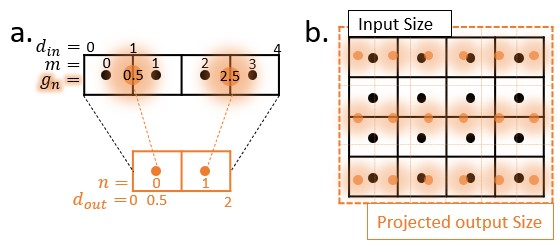
\includegraphics[width=1.5\textwidth]{figs/fig_grid.jpg}
        %\vspace*{0.5cm}
        \begin{minipage}{1.5\textwidth}
            \captionsetup{oneside, margin={1cm,0cm}}
            \caption{{\it The projected grid.}}
            \label{fig:grid}
         \end{minipage}%
    \end{minipage}%
    \vspace*{-0.5cm}
\end{figure}



\textbf{Block 2 -- Neighbors extraction:} For each grid point \varbold{$\textbf{g}_n$}, we now extract all its discrete nearest-neighbors $\varbold{\mathcal{N}[\textbf{n}]}$ \ben{from} $I$. These are all the input `pixels' centers within the support of the continuous kernel $\mathcal{K}_\theta$. This information is captured by a tensor of order 6 (blue tensor in Fig.~\ref{fig:overview}),  with shape $[N,1,C_{in},K,H',W']$ where K is the number of discrete neighbors in the kernel support. The second singleton dimension is for convenience in the next steps. We further need to extract the distances of each sub-`pixel' grid point \varbold{$\textbf{g}_n$} (of an output `pixel' {$\textbf{n}$}),  to all its discrete neighbors  ${\textbf{m}}\in I$. These distances $\varbold{\mathcal{D}[\textbf{n,m}]}$ are kept in a tensor $\varbold{\mathcal{D}}$ (shown in cyan in Fig.~\ref{fig:overview}), whose shape is $[K,2,H',W']$.

% Given a standard CNN input Tensor with dimensions Batch-size, Channels, Height and Width: $[N,C_{in},H,W]$.  We predefine support size (not necessarily an integer) for the continuous kernel $\mathcal{K}_\theata$. For each projected-grid point $\textbf{g'}$ we extract both values and distances to all input `pixels' within the kernel support. This stage produces a tensor consisting of all the neighbors values for each output `pixel'. This forces us to add a fifth dimension to the Neighbors tensor- the neighbors dimension. We actually extend this tensor to have 6 dimensions for convenience in the next stage, so the final shape is $[N,1,C_{in},K,H',W']$ where K is the number of neighbors in the kernel support. The Tensor of distances is shaped as a standard 2d CNN tensor, Its dimensions are: $[K,2,H',W']$. We use the batch dimension to distinguish between different neighbors. The second (channel) dimension is 2 to describe horizontal and vertical distances. Note that for simplicity, Fig.~\ref{fig:overview} depicts a case where $N=1, C_{in}=1$ and only the three last dimensions of the tensor are apparent.

% \textbf{Stage 3- Calculate weights:} The weights $\varbold{\mathcal{W}}$ are produced by the learnable model $\varbold{\mathcal{K}_\theta}$ applied to the distances tensor $\varbold{\mathcal{D}}$. 
\textbf{Block 3 -- Calculate weights:} The weights are produced by a learnable model $\varbold{\mathcal{K}_\theta}$, which is applied to the distances tensor:
%$\varbold{\mathcal{D}}$:
$\varbold{\mathcal{W} = \mathcal{K}_\theta \big\{ \mathcal{D}\big\}}$ (similarly to \cite{wang2018deep}).
A weight is assigned to connect between each output `pixel' and all its discrete input neighbors. Therefore, the weight tensor $\varbold{\mathcal{W}}$ will have a shape of $[1,C_{out},C_{in},K,H',W']$ 
(red tensor in Fig.~\ref{fig:overview}). 
%This tensor is marked in red in Fig.~\ref{fig:overview}. 
Its first singleton dimension is needed to match the size of the Neighbors tensor $\varbold{\mathcal{N}}$. As in standard conv, each output channel  $C_{out}$ is connected to all input channels $C_{in}$ through $\varbold{\mathcal{W}}$. We use a small neural network for $\varbold{\mathcal{K}_\theta}$ called the ``Internal-Net'' (marked in green in Fig.~\ref{fig:overview}). It is a simple CNN sequence of 1$\times$1 conv layers and ReLUs. This way every output `pixel' $\textbf{n}$ connects only to distances $\varbold{\mathcal{D}[\textbf{n}]}$ within its own set of discrete input neighbors. 

% The weights are produced by a learnable model which maps the distances calculated at stage 2 to corresponding weights for all the neighbors. This enforces consistency alongside expressivity. While each output `pixel' is calculated using a distinct local discrete kernel, all these local kernels are governed by the same underlying mapping function. We can choose to use a predefined fixed mapping, but we will usually use a learnable neural network, referred to as the internal-net. The input will be the distances tensor from preious stage. since we force the same mapping function to each output `pixel' we use several 1$\times$1 convolution layers and ReLUs in the internal-net. Consistency of the mapping to different neighbors is also enforced, since different neighbors are different instances in a batch. However, any model can be plugged to calculate the weights. Like in standard discrete convolutions, we have a set of continuous kernels, each maps all the input channels to an output channel. The weighted sum is actually taken not only over the neighbor values, but also over the input channels. Similarly to the neighbors tensor, the final weights tensor is of order 6: $[1,C_{out},C_{in},K,H',W']$ where the first dimension is the batch dimension which is always 1, to match the neighbors tensor.

\textbf{Block 4 -- Apply weights:} The final stage executes Eq.~\ref{eq:underlying} for the entire output tensor,
by multiplying the Weights tensor (red) with the Neighbors tensor (blue) and summing over all neighbors and input channels:
%. We simply multiply the Weights tensor (red) with the Neighbors tensor (blue) and sum over all the neighbors and input channels:
% For a given input feature-map $I$ of size $[N,C_{in},H,W]$, scale-factors $s_h, s_w$ and wanted shape $H',W'$ given at inference we finally get: 
\vspace*{-0.4cm}
\begin{align}
\varbold{I'}=
CC\{\varbold{I}\}= \sum_{c_{in}, k} \varbold{\mathcal{N}} \otimes \varbold{\mathcal{W}}
\end{align} 
with the following tensor shapes: 

$ \varbold{I'}:[N,C_{out},H',W'], \quad \varbold{\mathcal{N}}: [N,1,C_{in},K,H',W'], \quad \varbold{\mathcal{W}}:[1,C_{out},C_{in},K,H',W'] $

\subsection{Training and Generalization}
\label{sec:train}
CC is end-to-end trainable. The only trainable parameters of CC are $\varbold{\theta}$,  the parameters of $\varbold{\mathcal{K}_\theta}$. The gradient is propagated from the CC output through the weights tensor $\varbold{\mathcal{W}}$ to them. Gradients need to also be propagated to previous layers through the CC input. This is done easily through the neighbors extraction since it is just slicing (each neighbour neuron is actually a copy of an input neuron).

The output shape is determined by the shape of the grid $\varbold{{g}}$. Since $\varbold{\mathcal{K}_\theta}$ is a fully convolutional network, it can be applied to any spatial input size both at training and inference. This means that regardless of what sizes and scales we train on, a single CC, with a single set of parameters $\varbold{\theta}$ is applicable to any size and scale determined at real-time.

The input to  $\varbold{\mathcal{K}_\theta}$ is 
$\varbold{\mathcal{D}}$, which through the grid  $\varbold{{g}}$ depends only on the desired output scale \&
shape. Naturally, to generalize to many scales, we can sample various scales during training. However, being fully 1$\times$1 convolutional, $\varbold{\mathcal{K}_\theta}$ actually maps every 2D distance vector
%distance (two coordinates -- vertical and horizontal)
$\varbold{\mathcal{D}[\textbf{n,m}]}$ to a single value (weight) $\varbold{\mathcal{W}[\textbf{n,m}]}$. This means that $\varbold{\mathcal{D}}$ actually contains a huge batch of
inputs. This produces an interesting advantage: in almost all cases CC generalizes from one scale to any other scale. This happens as long as the diversity of distances in a single grid is reasonable. Eq.~\ref{eq:grid} suggests that if the scale is a rational number with a small numerator, 
then there exists only a small set of grid coordinates, and consequently a small set of unique distances $\varbold{\mathcal{D}[\textbf{n,m}]}$. For example, for $s=\nicefrac{1}{2}$ and a kernel with support of 2$\times$2, we get:
%\rightarrow 
$\varbold{\mathcal{D}[\textbf{n}]} = \Big\{(-\nicefrac{1}{2},-\nicefrac{1}{2}), 
(-\nicefrac{1}{2},\nicefrac{1}{2}), 
(\nicefrac{1}{2},-\nicefrac{1}{2}), 
(\nicefrac{1}{2},\nicefrac{1}{2})
\Big\} \ \ \varbold{\forall \textbf{n}}$, which will not generalize to other scales/distances. In other words, generalization occurs over the distribution of distances $\varbold{\mathcal{D}}$  between the grid points and `pixel' centers. If this distribution collapses to a small set of possibilities, then such generalization is damaged. However, training with a \emph{randomly} selected float scale-factor will give a huge diversity of sub-`pixel' distances in $\varbold{\mathcal{D}}$, hence will be able to generalize with very high probability to any other scale factor.
%\michal{Is this still true for large gaps between the train-scale  and the test-scale? After all, this will lead to a large difference in support size of K}. \assaf{supprt size of K is independent of the scale} 
Empirical evaluation of this property is described in the experiments section and in Fig.~\ref{fig:generalize}.
%\michal{Reference to Fig. 7 broken}
% \textbf{Cross-scale generalization:} Since the learning model $\mathcal{K}_\theta$ is unaware of the scale, it can be trained to one scale and generalize to another, under reasonable conditions. the scale trained on, cannot be a special case that collapses back to convolution, or a rational number with a denominator that is too small. In other words, generalization occurs over the distribution of distances between the grid and `pixel' centers. If this distribution collapses to a small set of possibilities then such generalization is damaged. A randomly selected float scale-factor will be able to generalize with probability ~1. 


% \textcolor{red}{
% \subsection{Training the CC-layer for dynamic scale generalization}
% \begin{itemize}[leftmargin=0.7cm]
% \item Please explain how to train the CC-layer so that it can generalize at test-time to any desired scale and shape.
% \item Please stress that although we use many scale/shape augmentations of the output layer, this is still a single trained network (as opposed to training multiple different networks, each for a different fixed output scale/shape). This is obvious to us, but may be a natural misconception of the reviewers, so it is worth stressing. Better safe than sorry...
% \end{itemize}
% }